\chapter{Representation of Environments}

\textbf{Author: Fabian Kleinrad} 

This chapter is going to concern itself with the critical intersection of physical and digital space. Fundamental for autonomous navigation to work are means for the algorithm to observe its surrounding. In order to accomplish a translation from physical space to a medium tailored towards information propagation, a SLAM algorithm, which is described in detail in chapter \ref{chapter:slam}, is being used. These following sections are going to explore the data, which is the output of the mapping phase and input into the path planning phase.

\section{Abstract Environments}

Abstraction being the process of reducing an Object to the information needed for further processing. In conjunction with autonomous navigation this principle is ubiquitous. Due to restriction in terms of computational space and time, a simplification of complex compounds is needed. Such a loss of information naturally happens when using equivalent hardware to process ones surroundings.\newline
In order for autonomous navigation to work it is necessary for the computer to know the existence and position of objects surrounding the to be navigated vessel. This information can be provided or in case of using a SLAM algorithm self-taught. SLAM reduces the environment to positions in a 2 or 3 dimensional space. The algorithm is then left with an assortment of positions relative to the starting point, which is represented by the coordinate origin. To make use of this information is imperative to know the position of the robot in this abstracted space.\newline
With this approach to let the of letting the algorithm perceive the environment it guarantees an efficient and cost effective computation. By reducing obstacles to only the properties needed to avoid them unnecessary complexity is being circumvented.      

\section{Representation in Autumn}
To be able to utilize the information provided, there need to be the capability of bundling data into a tried and tested format, that enables easy access and reliable accuracy.\newline
Autumn uses the occupancy grid and point cloud as means to represent the data acquired in the mapping stage. The occupancy grid serves its purpose in a 2 dimensional environment, where as on the contrary the point cloud is utilized in 3 dimensional use cases.

\subsection{Occupancy Grid}
An occupancy grid is used for a 2-dimensional representation of the environment. Hereby in case of an occupancy grid, a grid structure is being overlaid over the environment. Therefor it is possible to discretize the world into cells. Each cell contains information about the probability of being occupied. In this context the assumption is made, that cells can either one of the two states. Thus it allows for a simplification of algorithms needed to update such data structures, because with this assumption it allows for the use of binary random variables. Grid cells which are for certain occupied are represented by 1, which relates to the 100 percent probability of being occupied. Contrary free cells are described by a 0 percent probability of being occupied. Visually these features are displayed by coloring the cells black and white and every probability in between.\footcite{OccupancyGridMaps2020}

\begin{figure}[h]
	\centering
	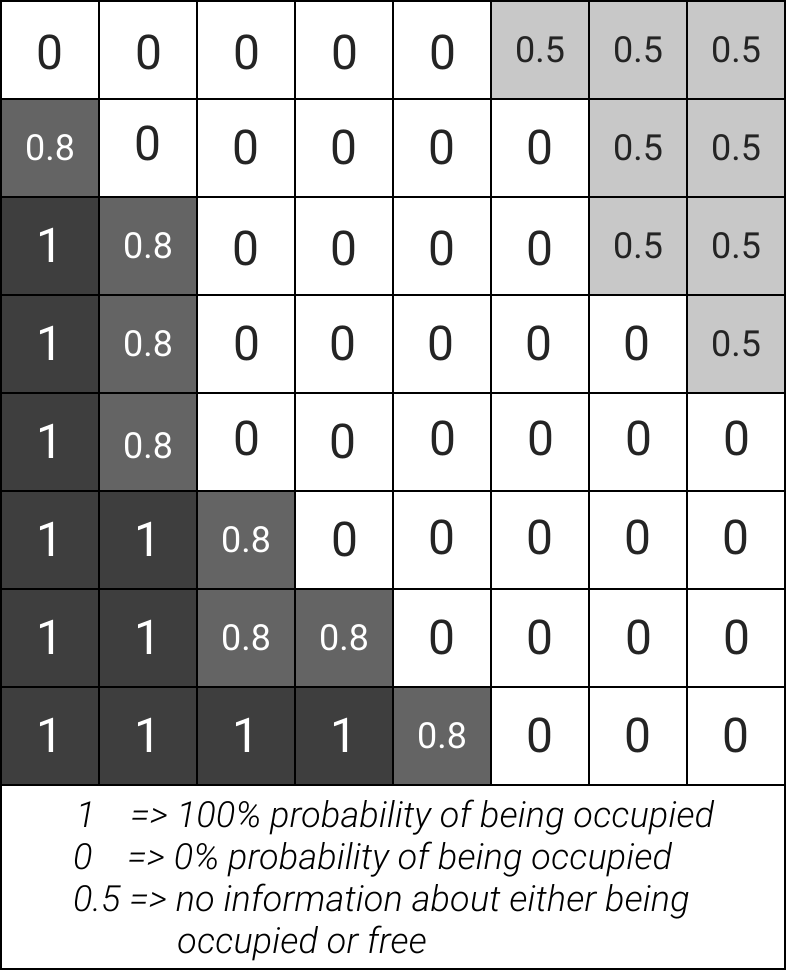
\includegraphics[width=0.5\linewidth]{img/OccupancyGridCells}
	\caption{Visual depiction of probability values in an occupancy grid map.}
	\label{fig:abstract_environments_occupancyCells}
\end{figure}

To add to the simplicity of the data structure and lower the time needed to update, two additional assumptions are made. The occupancy grid as well as many other assume a static world, which entails that occupied cells stay that way as well as their unoccupied equivalent. Secondly cells are viewed as individuals with know influence to their neighboring cells. This simplifies the calculations of probabilities, because of it the probability is the product of probability of single sensor readings.\footcite{uni-freiburgOccupancyGridMaps2020}

\subsection{Voxel Grids}

When familiar with the concept of an occupancy grid, it would appear that adding a dimension would solve the problem of 3 dimensional representation.
Using an occupancy grid in such an use case would be called a voxel grid. Hereby the environment isn't subdivided into 2 dimensional planes, also referred to as cells, but into cubes. The basic principle of the occupancy grid stays the same. Adding this additional dimension accentuates a drawback that accompanies the concept of occupancy grids. When working with occupancy grids the space needed to store this kind of structure grows linearly with the amount of cells. Now using it in a 3 dimensional context makes larger scans hard to maintain and inefficient to work with particularly in a real-time navigation scenario.\footcite{uni-freiburgOccupancyGridMaps2020}

\subsection{Point Cloud}
The most wide spread data structure for storing 3 dimensional environments is the Point Cloud. In contrast to its adversaries, it stores only information that is known. The drawback of the voxel grid is hereby minimized. Point Clouds store points in 3 dimensional space, these points represent an estimation of a point on a surface of an object, derived from sensor readings and the position these readings took place. Therefor a Point Cloud is a accumulation of various points that together represent the boundaries in which collision free navigation can take place.
Additionally to the positional information stored in these points, they can also contain color information and luminescence values.\footcite{tech27PointCloud2018}\newline
By discarding a strict grid structure, which intern decreases the spacial requirements, also increases the complexity in working with this kind of data structure. Almost always are point clouds in conjunction with robotics used along with the point cloud library.

\subsubsection{PCL}
The Point Cloud Library simplifies working with a point cloud data structure. PCL is an free library supporting point clouds of any dimension. It is written for optimal performance and offers a variety of 3d processing functionality. These include filtering, segmentation, feature estimation, etc. Furthermore PCL is fully integrated into ROS, which means specific functionalities are packages into nodelets which can be added to fit the underlying use case.\footcite{ConselhoNacionaldeDesenvolvimentoCientificoeTecnologico1995}

\section{Abstracted Environments in Autumn}
Autumn contains two different path planning packages catering to different dimensional environments. When using a drone 3 dimensional path planning is necessary to benefit from the usage of an aerial vehicle. Therefor the "autumn\_pathfinding" is used, based on a point cloud. Additionally the package "autumn\_pathfinding\_2D" uses an occupancy grid and thus is appropriate for situations where the third dimension can't be utilized.\newline
Through the use of ROS, explained in detail in chapter \ref{chapter:ros}, this modular approach is made possible. The Point Cloud and Occupancy Grid data type are integrated into ROS and as such universally applicable.   

\begin{figure}[h]
	\centering
	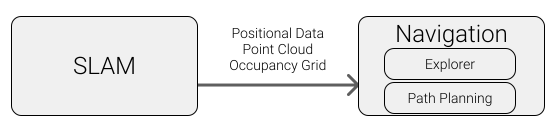
\includegraphics[width=0.8\linewidth]{img/EnvironmentTransfer}
	\caption{Excerpt of the Autumn-Life-Cycle. Lifespan of point cloud and occupancy grid. Created in the SLAM stage, published as a topic and used in the navigation stage.}
	\label{fig:abstract_environments_enviromentTransfer}
\end{figure}

\subsection{autumn\_pathfinding\_2D}
The package "autumn\_pathfinding\_2D" subscribes to an topic, published from the slam node, which carries a nav\_msgs/OccupancyGrid. This being a standardized data type for occupancy gird maps. It consists of an header of type std\_msgs/Header, which contains a sequence number, timestamp and frame id, that are used for identifying individual messages. Additionally meta data of the map along with the current data contained in an int8 array is transferred over this topic.\footcite{rosNavMsgsOccupancyGrid2021}\footcite{rosStdMsgsHeader2021}\newline
Upon receiving a new map and goal point, given that now current calculations are ongoing, the algorithm aligns a Cartesian coordinate system relative to the current position of the drone. From this point onward the access to the occupancy grid which is represented by the int8 array, happens through a function which takes x and y coordinates and maps it to the one dimensional array. This is essential to guarantee usability alongside performance.\newline
The coordinates get also adjusted based on the occupancy grid resolution. Benefits gained from such a procedure are that it is easy to check duplicate cells, because only whole cells can be represented. Another reason for it is the use of the cantor pairing function\footcite{Szudzik2017} which only works with natural numbers. The reason for using such a pairing function is to efficiently store and search for points.  
The underlying path planning algorithm, explained in detail in chapter \ref{chapter:path_planning}, isn't effected by the input data structure.       
The data array, holding occupancy information, contains per index a value between 0 and 100 or if the cell is unknown the value -1. The path planning algorithm works in a way that unknown cells with value -1 are taken as free cells. With this "free until proven occupied" mentality it allows for a more efficient exploration of a space.

\subsection{autumn\_pathfinding}
The 3 dimensional equivalent to the two dimensional path planning packages uses a point cloud in order to navigate the environment. This point cloud is published as a sensor\_msgs/PointCloud message type. This universal point cloud type contains a header with message specific information as well as an array of geometry\_msgs/Point32, which represent the individual points of the point cloud. The Point32 contains x, y and z attributes which represent the Cartesian coordinates.\footcite{rosGeometryMsgsPoint322021}\footcite{rosSensorMsgsPointCloud2021}\newline
Because of the difficulty of working with a three dimensional space represented by a one dimensional array, the point cloud library will be used. Same as the two dimensional variant, the algorithm of the three dimensional path planning accesses the data of the point cloud through a function which takes three coordinates and returns if an object exists at this position.\newline
Similar to the 2d solution, point coordinates get adjusted to a certain resolution. In this case it is not bound to the data type itself, because of the lack of structure in a point cloud. Instead the point resolution is chosen to guarantee best performance while retaining a high level of flexibility. This process of adjusting the resolution, can be understood as altering the size of cubes covering the space, like cells in an occupancy grid. This way there is a structure added to the otherwise unstructured set of points, which allows for the same implementation of the algorithm as in the two dimensional solution. 

